\documentclass{beamer}
\usepackage{hyperref}
\usepackage{amsmath}
\usepackage{multirow}
%\usepackage{minted}
\usepackage{alltt}


\usetheme{beaver}
\setbeamertemplate{footline}[page number]
\setbeamertemplate{navigation symbols}{}

\AtBeginSection{\frame{\sectionpage}}
\AtBeginSubsection{\frame{\subsectionpage}}

\defbeamertemplate{section page}{mine}[1][]{%
  \begin{centering}
    {\usebeamerfont{section name}\usebeamercolor[fg]{section name}#1}
    \vskip1em\par
    \begin{beamercolorbox}[sep=12pt,center]{part title}
      \usebeamerfont{section title}\insertsection\par
    \end{beamercolorbox}
  \end{centering}
}

\defbeamertemplate{subsection page}{mine}[1][]{%
  \begin{centering}
    {\usebeamerfont{subsection name}\usebeamercolor[fg]{subsection name}#1}
    \vskip1em\par
    \begin{beamercolorbox}[sep=8pt,center,#1]{part title}
      \usebeamerfont{subsection title}\insertsubsection\par
    \end{beamercolorbox}
  \end{centering}
}

%template for Q&A slide
\defbeamertemplate{section page}{questions}[1][]{%
	\begin{centering}
		{\usebeamerfont{section name}\usebeamercolor[fg]{section name}#1}
		\vskip1em\par
		\begin{beamercolorbox}[sep=12pt,center]{part title}
			\usebeamerfont{section title}\insertsection\par
		\end{beamercolorbox}
		\vskip1em
		Sachini Weerawardhana\\
		\texttt{sachini@cs.colostate.edu}\\
		\vskip1em
		Computer Science Department \\ 
		Colorado State University \\
		Fort Collins, CO 80524, USA\\
	\end{centering}
}



\title{Domain-independent Plan Intervention When Users Unwittingly Facilitate Attacks}
\author{Sachini Weerawardhana, Darrell Whitley, Mark Roberts}
\institute{Explainable AI Planning Workshop \\ ICAPS'19 \\Berkeley, CA, USA}
\begin{document}
\maketitle

%\begin{frame}{Outline}
%  \begin{itemize}
%   \item Introduction
%   \item Motivation
%   \item Problem
%   \item Learning to Intervene
%   \item Findings
%   \item Explaining Intervention
%   \item Future Work
%  \end{itemize}
%\end{frame}

\section{Introduction}\label{sec:intro}
When an agent is executing a plan to achieve some goal, it’s progress may be challenged by unforeseen changes such as an unexpected modification to the environment or an adversary subverting the agent’s
goal. In these situations, a passive observer intervening to help the agent reach it’s intended goal will be beneficial. Intervention is
different from the typical plan recognition problem because we assume the observed agent pursues desirable goals while avoiding undesirable states. The observer must (1) monitor actions/state unobtrusively to predict trajectories of the observed agent and (2) assist the observed agent to safely complete the task with timely interrupts.

We model online plan intervention in a competitive environment where three agents operate: (1) a human user, (2) an attacker (human or a software agent) and (3) an observer (a software agent) who will interrupt the user. The source of competition in the domain is either the attacker who leverages user's progress to achieve it's own goal or the user's uncertainty (e.g., hidden information, problem complexity). The user in the domain is pursuing a desirable goal while avoiding undesirable states. The observer, akin to the automated support system, acts as a cognitive assistant to the user.

Intervention needs to occur in different times during plan execution, based on which the user can plan to correct course or rely on the observer to make suggestions (e.g., counterplanning, alert and block action). In this work we focus on identifying critical actions, which if unchecked will definitely trigger the undesirable state. Intervention is useful in both online settings, where undesirable states may arrive incrementally (e.g., learning strategies in games) and in offline settings where observations are available prior to intervention (e.g.,troubleshooting execution).

We train a classifier with domain-independant features the observer uses to decide whether to intervene. We propose two methods: \textit{The Full method} uses a variation of the relaxed plan graph \cite{blum1997fast} to model the desirable, undesirable, and neutral states that are reachable at different depths. From the graph, we extract domain independent features: risk, desirability, distances remaining to desirable goal and undesirable states and  active landmarks (defined in Section \ref{sec:problemstatement} percentage. \textit{The Partial method} uses plan similarity metrics as features to identify risky actions without enumerating the full plan space. The classifier is then used to predict intervention on previously unseen observations.


The contributions of this paper include: (1) formalizing the online intervention problem, (2) introducing Full and Partial methods for estimating the criticality of the current state, (3) presenting an approach that learns to classify an observation as intervention or not, (4) presenting a causal model that explains intervention, and (6) introducing a new plan intervention benchmark domain called Rush Hour.

\begin{frame}{The Tale of Two Domains}
	\begin{figure}[t]
	\centering{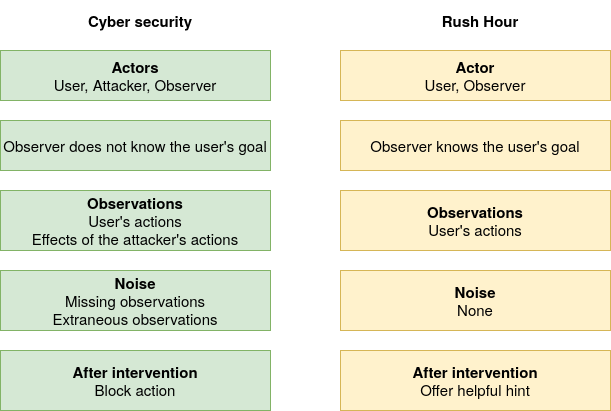
\includegraphics[width=4.5 in]{img/characteristics.png}}
	\label{fig:scenario}
\end{figure}

\end{frame}
\begin{frame}{Research Questions (1 of 2)}
\begin{itemize}
\item \textbf{1: What are the salient characteristics for deciding when to intervene}?
\begin{itemize}
\item When the user’s goals are known (Rush Hour)
\item When the user's goals are not known (Cyber-security)
\end{itemize}
\item \textbf{2: How to help task continuation following intervention}?
\begin{itemize}
\item Probe the search space
\item Tell the user about the probes, not the solution
\end{itemize}
\end{itemize}
\end{frame}

\begin{frame}{Research Questions (2 of 2)}
\begin{itemize}
\item \textbf{3: How to design tools to study intervention with human user participation}?
\begin{itemize}
\item Planning Domain Definition Language (PDDL) models for the two domains
\item Software tools to study human users in-situ.
\end{itemize}
\end{itemize}
\end{frame}
\begin{frame}{Undesirable States: Cyber-security Domain}

\begin{figure}[ht]
  \centering
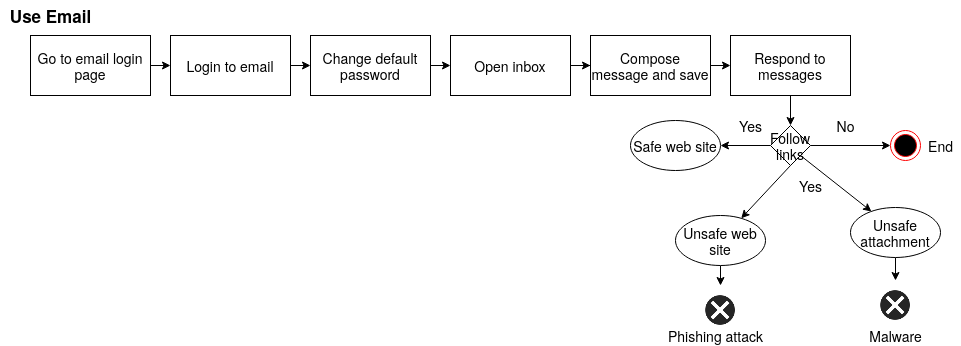
\includegraphics[width=\columnwidth, keepaspectratio=true]{img/Tasks.png}
\end{figure}

\end{frame}

\begin{frame}{Research Question 1: \\Salient characteristics for deciding when to intervene}
	\begin{figure}[!htb]
  \centering
  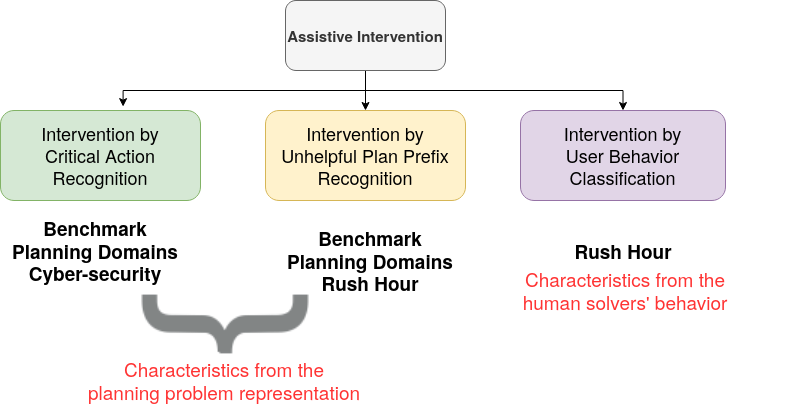
\includegraphics[width=\columnwidth, keepaspectratio=true]{img/breakdown.png}
\end{figure}
\end{frame}
\begin{frame}{Experimental Setup}
	\begin{itemize}
		\item Training
		\begin{itemize}
			\item Four benchmark domains
			\begin{itemize}
				\item {Blocks words, Navigator, IPC-grid+, Ferry}
			\end{itemize}
			\item 20 intervention problems for each domain
			\item Max 100 observation traces for each intervention problem
		\end{itemize}
		
		\item Testing
		\begin{itemize}
			\item 3 different instances of 20 intervention problems for each domain
			\item Max 10 observation traces for each intervention problem
		\end{itemize}
		
		\item Accuracy measures
			\begin{itemize}
				\item Predict intervention in testing dataset using the trained model
				\item compute True-positive, False-positive, True-negative, False-negative rates 
			\end{itemize}
	\end{itemize}
\end{frame}


\begin{frame}{Results}
	\begin{itemize}
		\item Accuracy in predicting intervention online
		\begin{itemize}
			\item Very high TPR, TNR 
			\item Very low FPR, FNR
		\end{itemize}
		\begin{figure}[p]
			\centering{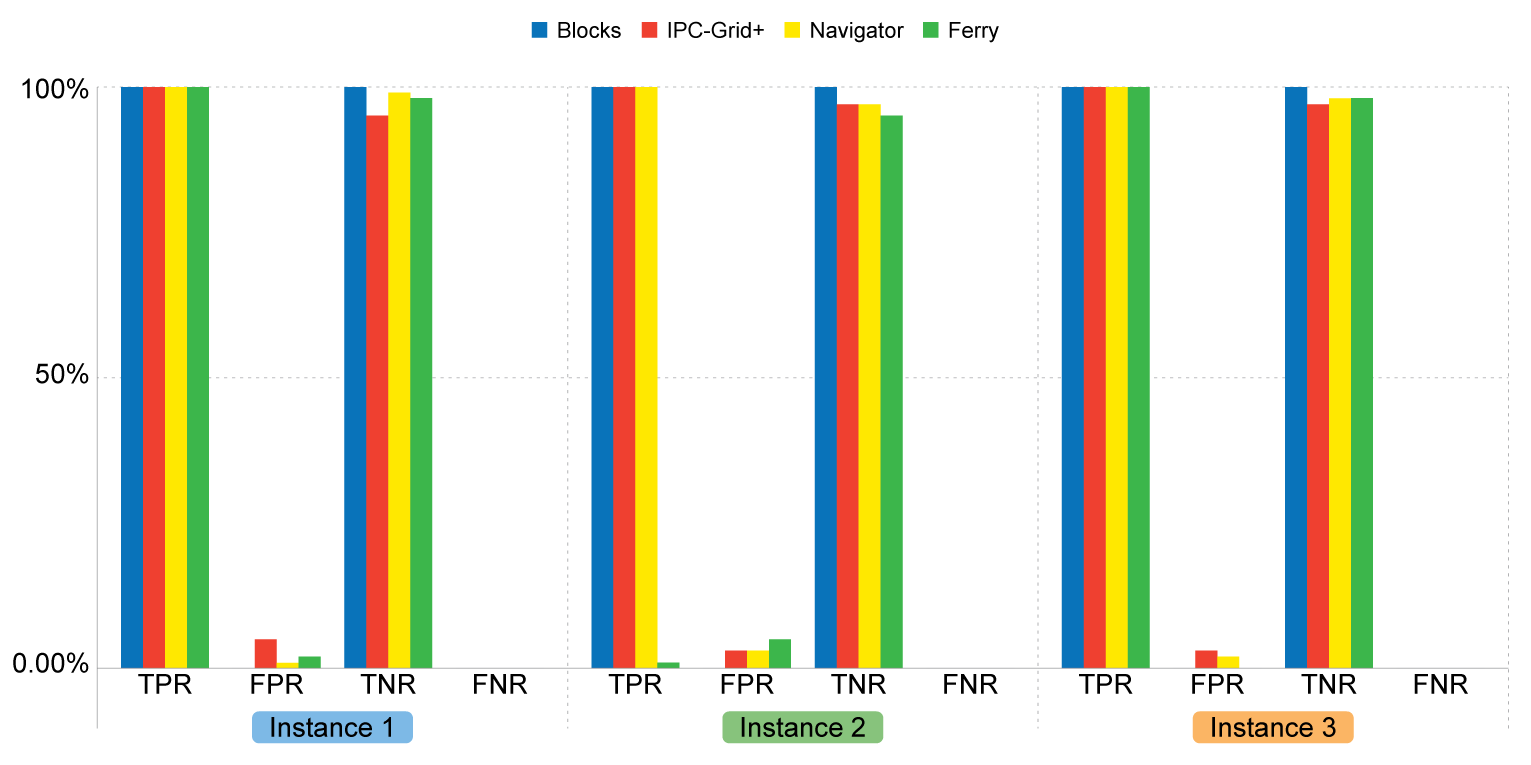
\includegraphics[width=3.5 in]{accuracy.png}}
			\label{fig:accuracy}
		\end{figure}
	\end{itemize}
\end{frame}

\begin{frame}{Explaining Intervention}
	\begin{itemize}
	\item Decision Trees
		\begin{figure}[p]
			\centering{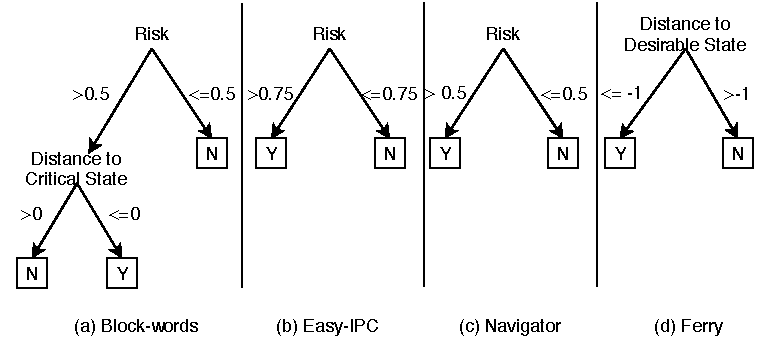
\includegraphics[width=2.5 in]{tree.pdf}}
			\label{fig:dt}
		\end{figure}
		%\item Use decision trees to derive a rule base to explain intervention
\begin{table}[]
\centering
\resizebox{\framewidth}{!}{%
\begin{tabular}{|l|l|l|l|}
\hline
\multicolumn{1}{|c|}{Domain} & \multicolumn{1}{c|}{Rules}                                 & \multicolumn{1}{c|}{Mapping}  & \multicolumn{1}{c|}{Effect}                                               \\ \hline
\multirow{4}{*}{BlocksWords} & Risk \textless{}= 0.5                                      & ``No risk of triggering undesirable state"   & N                                   \\ \cline{2-4} 
                             & Risk \textgreater 0.5                                      & ``Some risk of triggering undesirable state"   & -                                \\ \cline{2-4} 
                             & Dist. to Critical \textgreater 0 AND Risk \textgreater 0.5 & ``Somewhat high risk but undesirable state is not imminent" & N                   \\ \cline{2-4} 
                             & Dist. to Critical \textless{}= 0 AND Risk \textgreater 0.5 & ``Very high risk and undesirable state is imminent" & Y                           \\ \hline
\multirow{2}{*}{IPC-Grid+}   & Risk \textless{}=0.75                                      & ``No risk of triggering undesirable state"       & N                              \\ \cline{2-4} 
                             & Risk \textgreater 0.75                                     & ``Very high risk of triggering undesirable state"  & Y                            \\ \hline
\multirow{2}{*}{Navigator}   & Risk \textless{}= 0.5                                      & ``No risk of triggering undesirable state"        & N                             \\ \cline{2-4} 
                             & Risk \textgreater 0.5                                      & ``Very high risk of triggering undesirable state"   & Y                           \\ \hline
\multirow{2}{*}{Ferry}       & Dist. to desirable \textless{}= -1                         & ``Undesirable state is not imminent" & N \\ \cline{2-4} 
                             & Dist to desirable \textgreater -1                          & ``Undesirable state is imminent and occurs before reaching the desirable goal"           & Y                                 \\ \hline
\end{tabular}%
}
\end{table}
	\item $[$\texttt{Observation}$]$ $[$\texttt{Effect}$]$ because $[$\texttt{Mapping}$]$\\
{\small $[$\textsc{stack B A}$]$ $[$was interrupted$]$ because $[$very high risk and undesirable state is imminent$]$}
	\end{itemize}
\end{frame}


\begin{frame}{Future Work \& Summary}
	\begin{itemize}
	
	\item Summary
		\begin{itemize}
		\item Intervention is as important as recognition
		\item Formalize the intervention problem in competitive domains and train a decision tree using domain-independant features to identify critical actions
		\item Explain intervention using natural language templates generated from a rule base
		\end{itemize}
		
		\item Future Work
		\begin{itemize}
			\item Adopt different sampling strategies and new features to handle large domains (search and rescue)
			\item Relax optimality constraints, uncertainty in the environment and threat models
			\item Integrating causality to explanations and user studies
		\end{itemize}
		
	\end{itemize}
	
\end{frame}

	


\setbeamertemplate{section page}[questions]
\section{Questions?}
\end{document}